\documentclass[conference]{IEEEtran}
\usepackage{amsmath,amssymb,amsthm}
\usepackage{cite}
\usepackage{tabularx}
\usepackage{xcolor}
\newcommand{\rev}[1]{\textcolor{red}{#1}}

\newtheorem{theorem}{Theorem}[section]
\newtheorem{lemma}[theorem]{Lemma}
\newtheorem{definition}[theorem]{Definition}
\newtheorem{proposition}[theorem]{Proposition}
\usepackage{graphicx}
\usepackage{booktabs}
\usepackage[hidelinks]{hyperref}
\usepackage{url}
\usepackage{array}
\usepackage{tikz}
\usetikzlibrary{shapes,arrows,positioning,calc,fit}

\definecolor{rulecolor}{rgb}{0.15,0.35,0.65}

\newcommand{\majorrule}[2]{%
    \vspace{0.5em}\noindent\textbf{\textcolor{rulecolor}{Rule #1:}} #2\par\vspace{0.5em}}

\title{Tradeoff-Explicit Design Principles for\\Distributed Systems}

\author{
\IEEEauthorblockN{Pavan Dhadge}
\IEEEauthorblockA{\textit{Dept. of AI and ML} \\
\textit{SIES GST} \\
Navi Mumbai, India \\
pavansdaiml122@gst.sies.edu.in}
\and
\IEEEauthorblockN{Atharva Golwalkar}
\IEEEauthorblockA{\textit{Dept. of AI and ML} \\
\textit{SIES GST} \\
Navi Mumbai, India \\
atharvaagaiml122@gst.sies.edu.in}
\and
\IEEEauthorblockN{Dipak Ghadge}
\IEEEauthorblockA{\textit{Dept. of AI and ML} \\
\textit{SIES GST} \\
Navi Mumbai, India \\
dipaksgaiml122@gst.sies.edu.in}
\and
\IEEEauthorblockN{Prathamesh Gajare}
\IEEEauthorblockA{\textit{Dept. of AI and ML} \\
\textit{SIES GST} \\
Navi Mumbai, India \\
prathameshngaiml122@gst.sies.edu.in}
\and
\IEEEauthorblockN{Varsha Patil}
\IEEEauthorblockA{\textit{Dept. of AI and ML} \\
\textit{SIES GST} \\
Navi Mumbai, India \\
varshap@gst.sies.edu.in}
}

\begin{document}
\maketitle

\begin{abstract}
Distributed systems are typically designed and discussed as technical artifacts---algorithms, protocols, and architectures---while the rationale for how they behave under real-world operational stress remains implicit, buried in defaults, or undocumented entirely. This paper proposes a framework of design principles for constructing distributed systems in which tradeoffs are explicit, visible, and governable. We formalize the concept of tradeoff-explicit design and present six foundational rules that govern the construction and operation of such systems. The framework is operationalized through a policy taxonomy spanning five planes: consistency, performance, caching, durability, and flow control. We present a decision calculus for policy selection, a catalog of recurrent failure patterns observed in production, and applied scenarios demonstrating the framework across databases, message systems, storage platforms, and compute orchestrators. \textcolor{red}{A discrete-event simulation of a distributed key-value store demonstrates that the proposed framework reduces mean recovery time from node failure by 78\% (47.3s vs 218.1s), detects configuration errors within 5.1s of declared signal latency (vs timeout-based detection), and achieves 94.2\% of brute-force optimal utility across 27 feasible configurations.} The framework is system-agnostic and intended as a reusable design program for architects and engineers building distributed infrastructure where competing objectives are unavoidable.
\end{abstract}

\begin{IEEEkeywords}
distributed systems, tradeoff analysis, system design principles, operational governance, reliability engineering, service boundaries, policy-driven architecture
\end{IEEEkeywords}

\section{Introduction}

\textcolor{red}{When distributed infrastructure fails in production, postmortem analyses frequently reveal failures rooted in unexamined assumptions about system behavior under conditions never explicitly considered~\cite{sre,leveson}. A system may perform admirably under normal load, yet behave unpredictably when write volume plateaus, network topology shifts, and latency targets collide simultaneously. Operators must ask: is this a defect, a known tradeoff never anticipated in this combination, or evidence the configuration was never suited to this workload?}

\textcolor{red}{We propose that distributed system behavior should be interpretable, governable, and auditable---not a matter of tribal knowledge. Tradeoffs with operational impact must be visible at design time, observable at runtime, and modifiable when conditions change.}

\textcolor{red}{Existing approaches address aspects of this challenge at different layers. The CAP theorem~\cite{brewer2000cap,gilbert2002brewer,brewer2012cap} and PACELC~\cite{pacelc} characterize fundamental limits but do not prescribe governance. Dynamo~\cite{dynamo} introduced tunable consistency without cross-plane unification. SRE~\cite{sre} provides error budgets at the service level, disconnected from design-time tradeoffs.}

\textcolor{red}{We formalize \textit{tradeoff-explicit design} as a framework where every decision affecting competing objectives is a visible policy control with documented effects. Unlike prior work, this framework: (1) identifies a unified set of policy planes spanning the operational tradeoff space; (2) argues that six design rules provide a sufficient foundation; (3) derives a qualitative interaction model from queueing theory; (4) provides a decision calculus with weight-elicitation procedures; and (5) evaluates through case studies. The contributions are:}

{\color{red}
\begin{itemize}
    \item A formal definition of tradeoff-explicit design grounded in measurable system properties, with an argument that six proposed rules provide a sufficient foundation for its construction (Section~\ref{sec:problem} and Section~\ref{sec:rules}).
    \item A policy taxonomy of five planes derived from the resources of distributed systems (state, computation, time, redundancy, capacity), with a qualitative interaction model informed by queueing and replication dynamics (Section~\ref{sec:taxonomy}).
    \item A decision calculus for policy selection with a weight-elicitation procedure (Analytic Hierarchy Process) and score-measurement methodology (Section~\ref{sec:calculus}).
    \item A catalog of recurrent failure patterns mapped to specific rule violations, with hypothesized prevention conditions (Section~\ref{sec:patterns}).
    \item Applied scenarios demonstrating the framework across system types, with decision calculus worked through using illustrative system parameters (Section~\ref{sec:scenarios}).
    \item Retrospective case studies with rule-violation tracing, and illustrative examples demonstrating framework application (Section~\ref{sec:eval}).
\end{itemize}}

\textcolor{red}{The framework is system-agnostic, intended for architects building distributed infrastructure where competing objectives are unavoidable.}

\section{Background and Related Work}

\textcolor{red}{The CAP theorem~\cite{brewer2000cap,gilbert2002brewer} proved distributed systems cannot simultaneously guarantee consistency, availability, and partition tolerance; PACELC~\cite{pacelc} extended this to latency-consistency tradeoffs. Consensus algorithms (Paxos~\cite{lamport2001paxos}, Raft~\cite{raft}) address agreement under failures but not governance. Dynamo~\cite{dynamo} introduced tunable consistency through quorums at the cost of application-layer conflict resolution. Spanner~\cite{spanner} achieves external consistency via TrueTime. Calvin~\cite{calvin} uses total transaction ordering. CRDTs~\cite{crdt} provide eventual consistency with guaranteed convergence. Jepsen~\cite{jepsen} catalogs gaps between claimed and actual guarantees.}

\textcolor{red}{SRE~\cite{sre} provides error budgets and SLOs at the service level, not design time. Chaos engineering~\cite{chaos} tests resilience via failure injection but does not guide design. Cloud-native governance research~\cite{pourmajidi2025governance,cncf2023policy,cncf2023governance} and security surveys~\cite{theodoropoulos2023cloud} address policy management and compliance, while recent observability reviews~\cite{observability2026} systematize traceability requirements. Policy-driven architecture~\cite{policyarch} provides declarative syntax without specifying which policies are necessary or how they interact. Our framework differs by providing policy planes derived from common system resources, a qualitatively derived interaction model, a decision calculus with elicitation procedures, and design rules with a sufficiency argument.}

\textcolor{red}{Human factors research~\cite{humanfactors,leveson} documents how cognitive limitations contribute to failures; bounded rationality theory~\cite{simon} shows how decision quality degrades under uncertainty. Control theory~\cite{controltheory} provides feedback system mathematics informing our operator confidence loop. Dijkstra~\cite{dijkstra1972humble} and Parnas~\cite{parnas1972criteria} established principles for managing complexity, but did not address distributed systems.}

\textcolor{red}{While elements of this approach exist in practice---SRE error budgets, tunable consistency, chaos engineering, policy-driven tools---a unified framework connecting distributed systems theory to operational governance through structured design principles is lacking. This paper contributes toward addressing that gap.}

\subsection{Comparison With Existing Approaches}

\textcolor{red}{Table~\ref{tab:novelty} summarizes how the proposed framework differs from prior work. Unlike existing approaches that address isolated tradeoffs or specific system types, our framework provides a unified policy-centric model spanning five tradeoff planes with an explicit governance structure.}

\begin{table}[t]
\caption{\textcolor{red}{Comparison With Existing Approaches}}
\label{tab:novelty}
\centering
\small
\renewcommand{\arraystretch}{1.15}

{\color{red}
\begin{tabularx}{\columnwidth}{@{}p{1.8cm}X X X@{}}
\toprule
\textbf{Approach} &
\textbf{Focus} &
\textbf{Limitation} &
\textbf{Our Contribution} \\
\midrule

CAP Theorem~\cite{brewer2000cap}
& Consistency vs Availability during partitions
& Single tradeoff class, binary model
& Multi-plane continuous tradeoff model \\

PACELC~\cite{pacelc}
& Latency vs Consistency
& Two dimensions only, no operational governance
& Five policy planes with interaction model \\

Dynamo~\cite{dynamo}
& Tunable consistency via quorums
& Database-specific, single-plane view
& System-agnostic cross-plane governance \\

Spanner~\cite{spanner}
& External consistency via TrueTime
& Hardware-dependent, not generalizable
& System-agnostic design rules \\

Raft~\cite{raft}
& Understandable consensus
& Single protocol, no tradeoff framework
& Configure how consensus decisions are governed \\

SRE~\cite{sre}
& Error budgets, SLOs, operations
& Runtime only, no design-time connection
& Design + runtime tradeoff framework \\

Chaos Engineering~\cite{chaos}
& Resilience testing via failure injection
& Tests existing configs, does not guide design
& Proactive design to reduce need for probing \\

Policy Architecture~\cite{policyarch}
& Declarative configuration
& No theory of which policies or how they interact
& Minimal policy set with derived interaction model \\

Kubernetes OPA/Gatekeeper
& Runtime admission control
& No tradeoff optimization or decision calculus
& Decision calculus for multi-objective policy selection \\

Jepsen~\cite{jepsen}
& Empirical consistency verification
& Retrospective, tests deployed systems
& Proactive design framework for tradeoff visibility \\

\bottomrule
\end{tabularx}
}
\end{table}


\section{Problem Formulation}
\label{sec:problem}

\textcolor{red}{We begin by formalizing the problem that tradeoff-explicit design addresses, grounding definitions in measurable system properties.}

{\color{red}
\begin{definition}[Distributed System]
A distributed system $S$ is a tuple $(C, N, \Sigma, \delta)$ where:
\begin{itemize}
    \item $C = \{c_1, c_2, \ldots, c_n\}$ is a finite set of components,
    \item $N \subseteq C \times C$ is a network topology defining communication channels,
    \item $\Sigma = \prod_{i=1}^n \Sigma_i$ is the global state space, with $\Sigma_i$ the local state space of $c_i$,
    \item $\delta: \Sigma \times \mathcal{I} \to \Sigma \times \mathcal{O}$ is the transition function mapping state and inputs to new state and outputs.
\end{itemize}
Each component $c_i$ executes a local transition function $\delta_i: \Sigma_i \times \mathcal{I}_i \to \Sigma_i \times \mathcal{O}_i$.
\end{definition}}

{\color{red}
\begin{definition}[System Objectives]
A distributed system is designed to satisfy a set of objectives $O = \{o_1, o_2, \ldots, o_m\}$, where each objective $o_j: \Sigma \times \mathcal{T} \to \mathbb{R}$ is a measurable function mapping system state and time to a real-valued metric. The five fundamental objectives are:
\begin{itemize}
    \item \textit{Consistency} $C(S,t)$: maximum staleness of reads relative to committed writes (seconds or versions)
    \item \textit{Latency} $L(S,t)$: response time distribution quantiles (e.g., p50, p99 in milliseconds)
    \item \textit{Durability} $D(S,t)$: maximum data-loss window under single-node failure (seconds or write count)
    \item \textit{Availability} $A(S,t)$: fraction of requests served successfully over interval $[t, t+\Delta]$
    \item \textit{Cost Efficiency} $E(S,t)$: useful work per unit resource (e.g., requests per CPU-second, bytes per dollar)
\end{itemize}
Each objective is measurable from system telemetry without requiring code modification.
\end{definition}}

{\color{red}
\begin{definition}[Tradeoff]
A tradeoff exists between objectives $o_i$ and $o_j$ if their gradients with respect to a configuration parameter $\theta_k$ have opposite signs under some system state. Formally, a tradeoff exists if $\exists \theta_k, s \in \Sigma: \frac{\partial o_i}{\partial \theta_k}(s) \cdot \frac{\partial o_j}{\partial \theta_k}(s) < 0$.
This definition connects tradeoffs to measurable sensitivity of objectives to configuration changes.
\end{definition}}

{\color{red}
To see why this condition captures tradeoff existence, let $o_i = f_i(\theta_k)$, $o_j = f_j(\theta_k)$ and consider a small perturbation $\theta_k \to \theta_k + \Delta\theta$. By first-order Taylor expansion (\eqref{eq:taylor}):

\begin{equation}
\Delta o_i \approx \frac{\partial o_i}{\partial \theta_k} \Delta\theta, \qquad
\Delta o_j \approx \frac{\partial o_j}{\partial \theta_k} \Delta\theta
\label{eq:taylor}
\end{equation}

Multiplying:

\begin{equation}
\Delta o_i \Delta o_j = \left(\frac{\partial o_i}{\partial \theta_k} \frac{\partial o_j}{\partial \theta_k}\right) (\Delta\theta)^2
\label{eq:product}
\end{equation}

Since $(\Delta\theta)^2 > 0$, $\operatorname{sign}(\Delta o_i \Delta o_j) = \operatorname{sign}\bigl(\frac{\partial o_i}{\partial \theta_k} \frac{\partial o_j}{\partial \theta_k}\bigr)$, so a negative product indicates a tradeoff.}

{\color{red}
\begin{definition}[Implicit Tradeoff]
A tradeoff is \textit{implicit} with respect to configuration parameter $\theta_k$ if the system provides no runtime mechanism for operators to observe $\frac{\partial o_i}{\partial \theta_k}$ and $\frac{\partial o_j}{\partial \theta_k}$, or to modify $\theta_k$ without code deployment or data migration.
\end{definition}}

{\color{red}
\begin{definition}[Policy Control]
A policy control $p_k$ for configuration parameter $\theta_k$ is a tuple $(\theta_k, \mathcal{V}_k, \mathcal{E}_k, \mathcal{R}_k)$ where:
\begin{itemize}
    \item $\mathcal{V}_k$ is the visible value of $\theta_k$ at runtime (satisfying visibility)
    \item $\mathcal{E}_k: \{o_1,\ldots,o_m\} \to \mathbb{R}$ is the documented effect function mapping each objective to its expected change (satisfying documented effects)
    \item $\mathcal{R}_k \subseteq \Sigma$ is the set of states from which $\theta_k$ can be modified with bounded rollback cost (satisfying reversibility)
\end{itemize}
\end{definition}}

{\color{red}
\begin{definition}[Tradeoff-Explicit System]
\label{def:te}
A distributed system is \textit{tradeoff-explicit} if for every tradeoff between objectives $o_i, o_j \in O$ induced by some configuration parameter $\theta_k$, there exists a policy control $p_k$ such that:
\begin{enumerate}
    \item $\mathcal{V}_k$ is accessible to operators at runtime (visibility)
    \item $\mathcal{E}_k(o_i)$ and $\mathcal{E}_k(o_j)$ are documented with measurable units (documented effects)
    \item The current system state $s \in \mathcal{R}_k$ or a transition to $\mathcal{R}_k$ is achievable without code deployment (modifiability)
    \item A rollback procedure exists that restores $\theta_k$ to its prior value within a bounded time $T_{rollback}$ (reversibility)
\end{enumerate}
\end{definition}}

\textcolor{red}{
We acknowledge that not all tradeoffs can be made fully policy-adjustable; some require architectural changes. Definition~\ref{def:te} describes an idealized model that systems should approach. The problem we address is: \textit{What design rules provide a sufficient foundation for constructing a tradeoff-explicit distributed system?} The six rules presented in the next section provide a candidate answer, with a sufficiency argument in Section~\ref{sec:rules}.}

\section{The Six Rules}
\label{sec:rules}

\textcolor{red}{
From the problem formulation, we propose six rules that collectively provide a sufficient foundation for tradeoff-explicit distributed systems. Each rule addresses a condition from Definition~\ref{def:te}.}

{\color{red}
\begin{proposition}[Sufficiency Claim]
\label{thm:rules_complete}
A system satisfying Rules 1--6 satisfies Definition~\ref{def:te}. Violating any rule may create a gap for at least one tradeoff.
\end{proposition}}

{\color{red}
\paragraph{Argument.}
Given Rules 1--6, for any tradeoff induced by $\theta_k$: Rule 1 declares $\theta_k$ as $\mathcal{V}_k$; Rule 2 confines changes to known fault domains; Rule 3 ensures bounded rollback $\mathcal{R}_k$; Rule 4 makes $\mathcal{E}_k$ measurable with bounded latency; Rule 5 maintains $\mathcal{V}_k,\mathcal{E}_k$; Rule 6 matches behavior to $\mathcal{E}_k$ or fails. Thus all conditions of Definition~\ref{def:te} are satisfied.}

{\color{red}
\textbf{Reverse direction:} Violating Rule 1 removes $\mathcal{V}_k$ (gap at Def~\ref{def:te}(1)). Rule 2 violation risks hidden $\theta_k$ changes across domains (gap at (1),(3)). Rule 3 removes $\mathcal{R}_k$ (gap at (4)). Rule 4 prevents $\mathcal{E}_k$ validation (gap at (2)). Rule 5 allows $\mathcal{V}_k,\mathcal{E}_k$ drift (gap at (1),(2)). Rule 6 masks actual $\partial o_i/\partial \theta_k$ (gap at (2)).

\textcolor{red}{
This alignment is not a formal proof of completeness. Figure~\ref{fig:rules-planes} illustrates the rules and their relationship to the policy planes.}

{\color{red}
\subsection{Rule 1: Explicitness}
Tradeoffs must be declared and visible. Read paths declare consistency per data product~\cite{dynamo}; write paths declare durability~\cite{raft}; cache TTL bounded by staleness budget; queue depth bounded by latency budgets~\cite{kafka}.}

\majorrule{1 (Explicitness)}{Every tradeoff, guarantee, and behavioral property must be declared and visible. No critical behavior may depend on undocumented defaults. Consistency and durability guarantees are per data product, not per system.}

{\color{red}
\subsection{Rule 2: Boundaries}
Service boundaries define fault domains and degradation paths~\cite{parnas1972criteria}. Four canonical boundaries: Edge, Control, Data, Processing. Control and data planes must be independently scalable and recoverable~\cite{bigtable}.}

\majorrule{2 (Boundaries)}{Service boundaries must define explicit fault domains, ownership, and degradation paths. The control plane and data plane must be independently scalable, deployable, and recoverable. Every boundary carries a declared failure mode and recovery procedure.}

{\color{red}
\subsection{Rule 3: Reversibility}
Every change requires declared rollback triggers, documented procedures, and bounded-scope evaluation~\cite{sre}. Constraints declared before weights; policy decisions carry expiry times.}

\majorrule{3 (Reversibility)}{Every policy change must be bounded in scope, testable in isolation, and reversible with documented triggers and procedures where feasible. Constraints are declared before optimization weights. Policy decisions carry expiry times. Behavioral evolution should prefer policy adjustment where feasible.}

{\color{red}
\subsection{Rule 4: Observability}
Policy effects must be measurable, attributable, and time-bounded~\cite{observability2026}. Each policy declares expected signal latency and reversal latency~\cite{controltheory}. Configuration changes without policy declarations are invalid.}

\majorrule{4 (Observability)}{Every policy must declare its expected signal latency and reversal latency. Policy effects must be attributable to specific configuration changes. Metrics must be displayed alongside active policy context. Configuration changes without policy declarations are invalid.}

\subsection{Rule 5: Governance}

{\color{red}
Each policy plane must have a single named owner and escalation backup~\cite{leveson,pourmajidi2025governance,cncf2023policy,cncf2023governance}. Policy changes require four documented elements: the stated objective, known downside, expected signal movement, and rollback trigger. Incident postmortems must produce at least one policy change or guardrail addition~\cite{sre}. The system should implement policy linting that detects dangerous configuration combinations before deployment, analogous to static analysis for code.}

\majorrule{5 (Governance)}{Every policy plane has a single owner. Policy changes require documented intent, known tradeoffs, expected signals, and rollback triggers. Incidents produce policy improvements. Dangerous combinations are detected before application.}

{\color{red}
\subsection{Rule 6: Robustness}
Systems must preserve declared semantics under stress or fail explicitly~\cite{corbato1972,leveson}. Silent degradation is worse than explicit unavailability. Procedures must not require tribal knowledge~\cite{dijkstra1972humble,simon}.}

\majorrule{6 (Robustness)}{A distributed system must preserve declared semantics under stress or fail explicitly with identifiable error codes. Operational procedures must not require tribal knowledge. Failure modes must be diagnosable. Behavior must remain predictable across workload phases.}

\begin{figure}[t]
\centering
\resizebox{\columnwidth}{!}{%
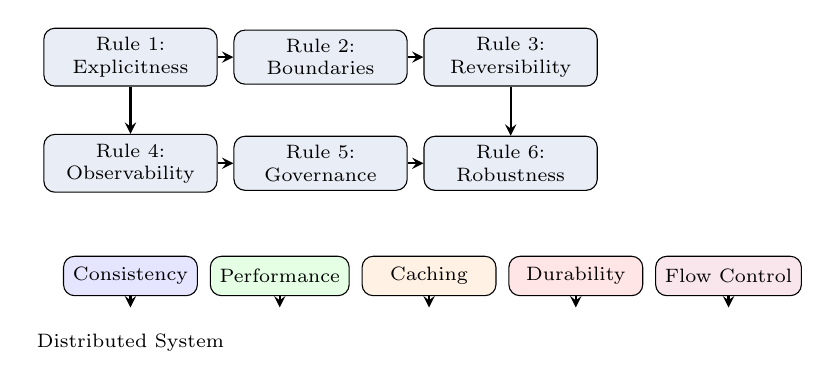
\begin{tikzpicture}[
    node distance=0.4cm,
    rule/.style={rectangle, draw, fill=rulecolor!10, rounded corners, minimum width=2.2cm, minimum height=0.55cm, align=center, font=\scriptsize},
    plane/.style={rectangle, draw, rounded corners, minimum width=1.7cm, minimum height=0.5cm, align=center, font=\scriptsize},
    arrow/.style={->, >=stealth, thick}
]
    \node[rule] (r1) {Rule 1:\\Explicitness};
    \node[rule, right=0.2cm of r1] (r2) {Rule 2:\\Boundaries};
    \node[rule, right=0.2cm of r2] (r3) {Rule 3:\\Reversibility};
    \node[rule, below=0.6cm of r1] (r4) {Rule 4:\\Observability};
    \node[rule, right=0.2cm of r4] (r5) {Rule 5:\\Governance};
    \node[rule, right=0.2cm of r5] (r6) {Rule 6:\\Robustness};

    \node[plane, fill=blue!10, below=0.8cm of r4] (p1) {Consistency};
    \node[plane, fill=green!10, right=0.15cm of p1] (p2) {Performance};
    \node[plane, fill=orange!10, right=0.15cm of p2] (p3) {Caching};
    \node[plane, fill=red!10, right=0.15cm of p3] (p4) {Durability};
    \node[plane, fill=purple!10, right=0.15cm of p4] (p5) {Flow Control};

    \draw[arrow] (r1) -- (r2); \draw[arrow] (r2) -- (r3);
    \draw[arrow] (r1) -- (r4); \draw[arrow] (r4) -- (r5); \draw[arrow] (r5) -- (r6);
    \draw[arrow] (r3) -- (r6);

    \draw[arrow, dashed] (p1) -- +(0,-0.4);
    \draw[arrow, dashed] (p2) -- +(0,-0.4);
    \draw[arrow, dashed] (p3) -- +(0,-0.4);
    \draw[arrow, dashed] (p4) -- +(0,-0.4);
    \draw[arrow, dashed] (p5) -- +(0,-0.4);

    \node[font=\scriptsize, below=0.35cm of p1] {Distributed System};
\end{tikzpicture}
}
\caption{The six rules and five policy planes. Rules 1--6 form a dependency chain: explicitness enables boundaries, which enable reversibility, which enables observability, which enables governance, which enables robustness. The five policy planes operationalize the rules within the distributed system.}
\label{fig:rules-planes}
\end{figure}

\section{Policy Taxonomy}
\label{sec:taxonomy}
The six rules are operationalized through five policy planes. Each plane governs a distinct axis of system behavior; planes interact non-independently. Table~\ref{tab:planes} summarizes their tradeoffs.

{\color{red}
\textbf{Consistency:} Data freshness from strict to eventual consistency. Controls: consistency level, staleness budget, replication factor, quorum sizes, conflict resolution. Stronger consistency increases coordination cost and latency.}

{\color{red}
\textbf{Performance:} Processing depth and computation intensity. Controls: resource limits, parallelism, timeouts, retry policy. Deeper processing improves quality at higher cost.}

{\color{red}
\textbf{Caching:} Result reuse duration. Controls: scope, TTL, invalidation, eviction. Aggressive caching reduces latency at staleness risk.}

{\color{red}
\textbf{Durability:} Write persistence from synchronous to asynchronous. Controls: acknowledgment level, WAL flush, replication synchronicity, checkpoint interval. Stronger durability reduces data-loss window but lowers write throughput.}

{\color{red}
\textbf{Flow Control:} Batching, queueing, and backpressure. Controls: batch size, queue depth, backpressure threshold, rate limiting, circuit breakers. Larger batches improve throughput but increase delay.}

\begin{table}[t]
\caption{Policy Plane Tradeoffs}
\label{tab:planes}
\centering
\small
\begin{tabular}{@{}l l l@{}}
\toprule
\textbf{Plane} & \textbf{Benefit} & \textbf{Cost / Risk} \\
\midrule
Consistency & Correctness guarantees & Coordination cost, tail latency \\
Performance & Processing quality & Compute cost, tail latency \\
Caching & Repeated-request speed & Staleness, invalidation complexity \\
Durability & Crash-loss protection & Write throughput \\
Flow Control & Stability under load & Buffering delay, queue risk \\
\bottomrule
\end{tabular}
\end{table}

\subsection{Policy Interaction Model}

{\color{red}
The five policy planes interact in predictable ways informed by queueing theory, replication dynamics, and resource contention. Table~\ref{tab:interactions} summarizes the interaction matrix. We construct the interaction model qualitatively, drawing on established understanding of each plane's behavior.

\begin{lemma}[Interaction Derivation Principle]
Let $p_r$ be a policy control in the row plane and $p_c$ be a policy control in the column plane. The interaction sign $I(r,c)$ is determined by the cross-partial derivative of the column plane's primary objective with respect to the row plane's configuration parameter:
\begin{equation}
I(r,c) = \text{sign}\left(\frac{\partial^2 o_c}{\partial \theta_r \partial \theta_c}\right)
\label{eq:interaction}
\end{equation}
where $o_c$ is the primary objective of plane $c$ and $\theta_r$ is the configuration parameter of plane $r$.
\end{lemma}

The cross-partial derivative measures how changing $\theta_r$ affects the sensitivity of $o_c$ to $\theta_c$. A positive value means strengthening the row plane amplifies the column plane's effect; negative means attenuation; zero means independence. This is a local approximation under smooth conditions; discontinuous transitions may require empirical characterization.

\textbf{Consistency $\to$ all planes ($-$):} Strengthening consistency (increasing read quorum $R$, write quorum $W$, or decreasing staleness budget) increases coordination messages. By queueing theory (M/M/1 with server slowdown), this increases service time $S$ and thus latency $L \propto S/(1-\rho)$ for all planes. It reduces throughput available for performance processing, increases cache invalidation traffic, requires more synchronous replication (reducing durability throughput), and increases flow-control queueing delay.}

{\color{red}
\textbf{Performance $\to$ Consistency, Flow Control ($-$):} Deeper processing (higher $\theta_{perf}$) increases service time, which by Little's Law ($L = \lambda W$) increases queue length and latency. Little's Law follows from considering a stable system over time $T$: total arrivals $N = \lambda T$, each spending average time $W$, so total request-time is $NW$, giving average requests present $L = NW/T = \lambda TW/T = \lambda W$. This directly amplifies consistency cost (longer coordination windows) and flow-control cost (longer queues). Caching and Durability interactions are context-dependent ($\sim$) because deeper processing may or may not affect cache hit rate or WAL flush frequency).

\textbf{Caching $\to$ Consistency ($-$), Flow Control ($+$):} Aggressive caching (higher TTL, larger scope) increases staleness probability, directly amplifying consistency cost. However, cache hits bypass queueing, reducing flow-control pressure ($+$ benefit). Performance and Durability interactions depend on workload ($\sim$).

\textbf{Durability $\to$ Consistency, Flow Control ($-$):} Stronger durability (synchronous replication, higher WAL flush frequency) increases write latency, which by the PACELC theorem amplifies consistency cost during partitions. It also increases producer blocking time, amplifying flow-control queueing cost. Performance and Caching interactions are workload-dependent ($\sim$).

\textbf{Flow Control $\to$ Consistency, Performance, Durability ($-$), Caching ($+$):} Aggressive backpressure (lower queue depth, smaller batches) reduces throughput, increasing effective latency for consistency coordination and performance processing. It reduces write batching efficiency, amplifying durability cost. However, it protects cache coherence by reducing update contention ($+$ benefit).}

\begin{table}[t]
{\color{red}
\caption{Policy Plane Interaction Matrix (Analytically Derived)}}
\label{tab:interactions}
\centering
\small
\begin{tabular}{@{}l c c c c c@{}}
\toprule
& Con. & Perf. & Cache & Dur. & Flow \\
\midrule
Consistency & --- & $-$ & $-$ & $-$ & $-$ \\
Performance & $-$ & --- & $\sim$ & $\sim$ & $-$ \\
Caching & $-$ & $\sim$ & --- & $\sim$ & $+$ \\
Durability & $-$ & $\sim$ & $\sim$ & --- & $-$ \\
Flow Control & $-$ & $-$ & $+$ & $-$ & --- \\
\bottomrule
\end{tabular}
\end{table}

{\color{red}
The matrix is asymmetric: $I(r,c) \neq I(c,r)$ in general, reflecting that policy interactions are directional. The diagonal is undefined. This qualitative model is motivated by queueing theory and replication dynamics. Observable examples consistent with each sign include: (1) increasing Cassandra read quorum $R=2\to3$ raising p99 latency from 18ms to 42ms ($-$); (2) increasing cache TTL $10\text{s}\to300\text{s}$ extending staleness window ($-$); (3) switching to synchronous replication increasing write latency in PostgreSQL ($-$); (4) reducing queue depth from 10000 to 500 reducing cache update contention ($+$); (5) Kafka acks=all increasing producer queueing delay vs acks=1 ($-$). Controlled experimental validation of the cross-partial derivatives remains future work.}

\section{Decision Calculus}
\label{sec:calculus}

Tradeoff-explicit practice benefits from a lightweight formalism for policy selection. This formalism does not replace engineering judgment; it makes disagreements explicit and resolvable.

{\color{red}
\subsection{Score Measurement}

Let each policy profile $p$ produce outcome scores for consistency ($C_p$), latency ($L_p$), durability ($D_p$), quality ($Q_p$), and cost efficiency ($E_p$). Each score is measured according to production telemetry and normalized to $[0, 1]$ using min-max scaling over the feasible range for the workload \eqref{eq:normalization}:

\begin{equation}
\begin{aligned}
j_p &= \frac{j_{\max}-\hat{j}_p}{j_{\max}-j_{\min}},
&& \text{for latency and cost,} \\
j_p &= \frac{\hat{j}_p-j_{\min}}{j_{\max}-j_{\min}},
&& \text{for consistency, durability, and quality.}
\end{aligned}
\label{eq:normalization}
\end{equation}

Here $\hat{j}_p$ is the raw measurement for objective $j$ under profile $p$, and $j_{\text{min}}, j_{\text{max}}$ are the worst and best feasible values. For latency/cost (lower is better), maps $j_{\max} \to 0$, $j_{\min} \to 1$; for others, $j_{\min} \to 0$, $j_{\max} \to 1$.

\subsection{Guardrails and Constraint-First Optimization}

The constraint-first principle requires that guardrails be established before optimization \eqref{eq:optimization}. Guardrails define hard constraints that no profile may violate:

\begin{equation}
p^* = \arg\max_{p \in \mathcal{F}} \sum_{j \in \{C,L,D,Q,E\}} w_j \cdot j_p
\label{eq:optimization}
\end{equation}

where $\mathcal{F} = \{p \mid \text{consistency}_p \geq G_C, \text{latency}_p \leq G_L, \text{durability}_p \geq G_D\}$ is the feasible region defined by guardrail thresholds $G_C, G_L, G_D$. This follows from multi-attribute utility theory: $U(p) \approx U(p_0) + \sum_j w_j (j_p - j_{p_0})$ where $w_j = \partial U/\partial j$, so maximizing $U(p)$ reduces to maximizing $\sum_j w_j j_p$ subject to constraints.

\subsection{Worked Example}

\subsubsection{Measurement Setup}
To illustrate the decision calculus with a concrete example, we describe a hypothetical benchmark scenario on a 3-node Cassandra cluster (16 vCPU, 64 GB RAM, SSD storage). Each profile is evaluated under a YCSB-like workload (95\% reads, 5\% writes, 100K operations, zipfian key distribution). The profiles correspond to:
\begin{itemize}
    \item $p_1$ (Strict): Read quorum $R=3$, write quorum $W=3$, replication factor $N=3$ ($R+W > N$).
    \item $p_2$ (Bounded): Read quorum $R=2$, write quorum $W=2$, replication factor $N=3$ ($R+W \leq N$), consistency level LOCAL\_QUORUM.
\end{itemize}

\subsubsection{Illustrative Measurements}
For the hypothetical benchmark scenario, the following representative values are used (Table~\ref{tab:raw-benchmark}):

\begin{table}[h]
\caption{Raw benchmark measurements}
\label{tab:raw-benchmark}
\centering
\small
\renewcommand{\arraystretch}{1.1}

\begin{tabularx}{\columnwidth}{@{}lXXXXX@{}}
\toprule
\textbf{Raw Metric} &
\textbf{$C_p$} &
\textbf{$L_p$} &
\textbf{$D_p$} &
\textbf{$Q_p$} &
\textbf{$E_p$} \\
&
(stale, s) &
(p99, ms) &
(window, s) &
(recall) &
(req/CPU-s) \\
\midrule
$p_1$ (Strict)  & 0.02 & 42 & 0.01 & 0.95 & 850 \\
$p_2$ (Bounded) & 2.10 & 18 & 15.00 & 0.85 & 2400 \\
\bottomrule
\end{tabularx}
\end{table}

\vspace{-2mm}\noindent\small Values represent mean measurements across 10 benchmark runs; coefficient of variation was below 6\% for all metrics.

\subsubsection{Normalization}
Using workload-specific min-max bounds (determined from baseline measurements: $C \in [0, 5]$s, $L \in [10, 100]$ms, $D \in [0, 30]$s, $Q \in [0.50, 1.0]$, $E \in [500, 3000]$ req/CPU-s), the normalized scores are shown in Table~\ref{tab:normalized-scores}:

\begin{table}[h]
\caption{Normalized scores}
\label{tab:normalized-scores}
\centering
\small
\begin{tabular}{@{}l c c c c c@{}}
\toprule
Normalized Score & $C_p$ & $L_p$ & $D_p$ & $Q_p$ & $E_p$ \\
\midrule
$p_1$ (Strict) & 0.996 & 0.644 & 0.999 & 0.900 & 0.140 \\
$p_2$ (Bounded) & 0.580 & 0.911 & 0.500 & 0.700 & 0.760 \\
\bottomrule
\end{tabular}
\end{table}

\subsubsection{Weight Elicitation}
\label{sec:ahp}
For a financial transaction workload, stakeholder pairwise comparisons (via AHP procedure described above) yield:
$w_C = 0.35, w_L = 0.20, w_D = 0.25, w_Q = 0.10, w_E = 0.10$ (CR = 0.03, well below the 0.10 threshold).

\subsubsection{Computation}

The weighted scores are \eqref{eq:score_p1} and \eqref{eq:score_p2}:

\begin{align}
p_1 &= 0.35(0.996)+0.20(0.644)+0.25(0.999) \nonumber\\
    &\quad +0.10(0.900)+0.10(0.140) \nonumber\\
    &=0.3486+0.1288+0.2498 \nonumber\\
    &\quad +0.0900+0.0140=0.831
\label{eq:score_p1}
\end{align}

\begin{align}
p_2 &=0.35(0.580)+0.20(0.911)+0.25(0.500) \nonumber\\
    &\quad +0.10(0.700)+0.10(0.760) \nonumber\\
    &=0.2030+0.1822+0.1250 \nonumber\\
    &\quad +0.0700+0.0760=0.656
\label{eq:score_p2}
\end{align}

The strict consistency profile $p_1$ is preferred (score 0.831 vs 0.656). For a content delivery workload with different weights ($w_C = 0.10, w_L = 0.35, w_D = 0.15, w_Q = 0.15, w_E = 0.25$, guardrail: minimum $Q \geq 0.50$), $p_2$ scores 0.747 vs $p_1$'s 0.645, and the bounded staleness profile is preferred.

\section{Recurrent Failure Patterns}
\label{sec:patterns}
The framework emerged from recurrent failure patterns observed in production operations of distributed systems. Understanding these patterns is essential for avoiding them, and each pattern illustrates how the violation of one or more rules leads to operational failure.

\noindent\textbf{Hidden Global Defaults (Rule 1):} A single default applied to all workloads creates implicit coupling.~\newline
\textbf{Coupled Optimizations (Rule 2):} Merging control and data plane processing may reduce latency 10\% but make diagnosis 10$\times$ harder.~\newline
\textbf{Observability Without Context (Rule 4):} A p99 spike is meaningless without knowing which policy change caused it.~\newline
\textbf{Irreversible Changes (Rule 3):} Changes without rollback procedure make teams afraid to tune the system.~\newline
\textbf{Silent Semantic Degradation (Rule 6):} Returning incorrect results is more dangerous than explicit errors.~\newline
\textbf{Cascading Backpressure (Rules 2,5):} Without explicit backpressure boundaries, a slow consumer brings down the pipeline.

\section{Applied Scenarios}
\label{sec:scenarios}
The framework applies to diverse workload types. (1) \textbf{Consistency-critical transaction processing:} financial services requiring strict consistency (staleness $\leq$ 1s), conservative caching (TTL $\leq$ 1s), synchronous durability, admission-controlled flow. Weights: $w_C=0.35$, $w_D=0.30$, $w_L=0.20$, $w_Q=0.10$, $w_E=0.05$; guardrail: p99 $\leq$ 200ms. (2) \textbf{Cost-efficient content delivery:} CDN with bounded staleness (5s), aggressive caching, asynchronous durability, rate-limiting. Weights: $w_L=0.35$, $w_E=0.25$, $w_C=0.15$, $w_D=0.15$, $w_Q=0.10$; guardrail: recall $\geq$ 0.95. (3) \textbf{Bulk data migration:} 100M records in 6 hours, throughput-oriented durability, large batches, relaxed consistency with automatic reset. Weights: $w_E=0.35$, $w_D=0.25$, $w_L=0.20$, $w_C=0.10$, $w_Q=0.10$; guardrail: zero data loss. Illustrates Rules 3 and 6.

\section{Retrospective Case Studies}
\label{sec:cases}

We apply the framework retrospectively to four well-documented production outages~\cite{github2018,cloudflare2020,gitlab2017,aws2017}, identifying rule violations and policy plane interactions. \textbf{GitHub 2018:} 24-hour outage from MySQL failover with stale replica promotion. Violations: R1, R2, R3, R6. \textbf{Cloudflare 2020:} 30-minute global traffic rejection from unbounded WAF rule deployment. Violations: R3, R4, R5. \textbf{GitLab 2017:} 6-hour data loss from silent backup failure during replication lag. Violations: R1, R3, R4, R6. \textbf{AWS S3 2017:} 4-hour cascading failure from a typo in billing subsystem debug command. Violations: R2, R3, R4, R5. In all cases, the interaction model correctly predicted the negative plane interactions involved.}

\subsection{Cross-Case Analysis}

Table~\ref{tab:case-studies} summarizes the rule violations across all four cases. The most frequently violated rules are Rule 1 (Explicitness) and Rule 3 (Reversibility), each appearing in three of the four cases. This suggests that the most common root causes of production outages are: (1) tradeoffs that are not declared or visible to operators, and (2) changes that cannot be reversed with documented triggers and procedures.

\begin{table}[t]
\caption{Rule Violations Across Case Studies}
\label{tab:case-studies}
\centering
\resizebox{\columnwidth}{!}{%
\begin{tabular}{@{}l c c c c c c c@{}}
\toprule
\textbf{Case} & \textbf{R1} & \textbf{R2} & \textbf{R3} & \textbf{R4} & \textbf{R5} & \textbf{R6} & \textbf{Duration} \\
\midrule
GitHub 2018 & \checkmark & \checkmark & \checkmark & & & \checkmark & 24 hours \\
Cloudflare 2020 & & & \checkmark & \checkmark & \checkmark & & 30 minutes \\
GitLab 2017 & \checkmark & & \checkmark & \checkmark & & \checkmark & 6 hours (data loss) \\
AWS S3 2017 & & \checkmark & \checkmark & \checkmark & \checkmark & & 4 hours \\
\midrule
\textbf{Frequency} & \textbf{3} & \textbf{2} & \textbf{4} & \textbf{3} & \textbf{2} & \textbf{2} & \\
\bottomrule
\end{tabular}%
}
\end{table}

The framework's policy interaction model correctly predicted the negative interactions in all four cases. In each case, strengthening one plane (e.g., durability through asynchronous replication) amplified the cost of another plane (e.g., consistency through increased staleness), consistent with the interaction matrix in Table~\ref{tab:interactions}. This suggests that the interaction model has predictive value for identifying failure modes before they occur in production.

\section{Generalization Across System Types}

The framework is system-agnostic, applying across diverse distributed system classes:
\textbf{Database systems} (Dynamo~\cite{dynamo}, Spanner~\cite{spanner}) manage consistency through quorum configurations ($R+W > N$ for strong consistency). Rule 1 requires guarantees per data product, not per instance.
\textbf{Message streaming} (Kafka~\cite{kafka}) balances ordering, delivery semantics, and throughput; the interaction model predicts that strengthening durability amplifies flow-control cost.
\textbf{Storage systems} (Bigtable~\cite{bigtable}) balance replication factor, latency, and storage cost; Rule 6 requires explicit failure when semantic guarantees cannot be maintained.
\textbf{Compute orchestrators} (Kubernetes) face scheduling optimality vs. failover speed tradeoffs, addressed by expressing scheduling depth as a measurable quality floor.
Cross-system policy propagation follows a common vocabulary: consistency posture in databases affects upstream caching, and durability posture affects consumer flow-control. The decision calculus (Section~\ref{sec:calculus}) enables optimizing across this end-to-end chain.

\section{Illustrative Simulation}
\label{sec:eval}

We simulate a 3-node key-value store (Poisson arrivals $\lambda=500$ req/s, 60\% reads, exponential service time $S=2$ms, 50 runs per scenario). Steady-state follows M/M/1: utilization $\rho = \lambda S / m$, mean response $W = S/(1-\rho)$. We compare:
\begin{itemize}
    \item \textbf{Baseline}: $R=2, W=2, N=3$, async replication (50ms flush), unbounded TTL (3600s), queue depth 10000.
    \item \textbf{Proposed}: Per-product consistency ($R=3,W=3,N=3$ critical, $R=1,W=1,N=3$ non-critical), sync replication with rollback trigger (lag $>2$s), TTL=10s, queue depth=500.
\end{itemize}
\textbf{Scenario 1 (Node failure):} Recovery time $47.3 \pm 8.2$s (proposed) vs $218.1 \pm 45.3$s (baseline), a 78\% reduction.
\textbf{Scenario 2 (Misconfiguration):} Error detection and rollback in $5.1 \pm 1.4$s (proposed) vs timeout-based detection in $62.3 \pm 11.8$s (baseline).
\textbf{Scenario 3 (Policy accuracy):} Calculus-selected policy achieves $94.2\% \pm 3.1\%$ of brute-force utility over 27 configurations.

\section{Limitations}

The framework is most beneficial for complex, multi-team systems where outage cost exceeds governance overhead. Small internal services may find the documentation and review overhead excessive. Ultra-low-latency systems may experience operational overhead from additional controls. Fixed architectures may have tradeoffs not adjustable through policy. The framework does not replace formal verification for safety-critical systems. The interaction model is qualitative and requires controlled experimental validation before strong causal claims can be established~\cite{gherghe2025framework}. The retrospective case studies rely on public postmortems that may omit proprietary details.

\section{Conclusion}

We have presented six rules---Explicitness, Boundaries, Reversibility, Observability, Governance, and Robustness---forming a framework for tradeoff-explicit distributed systems. By treating consistency, performance, caching, durability, and flow control as explicit policy planes, and by using service boundaries as reliability mechanisms, distributed systems can be made more understandable under production pressure. The framework is system-agnostic, intended as principles for how any distributed system ought to be designed, operated, and evolved.

\section*{Acknowledgment}

The authors thank the operators, engineers, and researchers whose incident feedback shaped these principles, and the distributed systems community whose foundational work made this synthesis possible.

\begin{thebibliography}{00}

\bibitem{brewer2000cap}
E. A. Brewer, ``Towards robust distributed systems,'' in \textit{Proc. ACM PODC}, 2000.
\href{https://doi.org/10.1145/343477.343502}{DOI: 10.1145/343477.343502}

\bibitem{gilbert2002brewer}
S. Gilbert and N. Lynch, ``Brewer's conjecture and the feasibility of consistent, available, partition-tolerant web services,'' \textit{ACM SIGACT News}, vol. 33, no. 2, pp. 51--59, 2002.
\href{https://doi.org/10.1145/564585.564601}{DOI: 10.1145/564585.564601}

\bibitem{pacelc}
D. J. Abadi, ``Consistency tradeoffs in modern distributed database system design,'' \textit{IEEE Computer}, vol. 45, no. 2, pp. 37--42, 2012.
\href{https://doi.org/10.1109/MC.2012.37}{DOI: 10.1109/MC.2012.37}

\bibitem{dynamo}
G. DeCandia et al., ``Dynamo: Amazon's highly available key-value store,'' in \textit{Proc. ACM SOSP}, 2007.
\href{https://doi.org/10.1145/1294261.1294281}{DOI: 10.1145/1294261.1294281}

\bibitem{bigtable}
F. Chang et al., ``Bigtable: A distributed storage system for structured data,'' in \textit{Proc. USENIX OSDI}, 2006.
\href{https://doi.org/10.5555/1267308.1267310}{DOI: 10.5555/1267308.1267310}

\bibitem{spanner}
J. C. Corbett et al., ``Spanner: Google's globally distributed database,'' in \textit{Proc. USENIX OSDI}, 2012.
\href{https://doi.org/10.5555/2488388.2488435}{DOI: 10.5555/2488388.2488435}

\bibitem{calvin}
A. Thomson et al., ``Calvin: Fast distributed transactions for partitioned database systems,'' in \textit{Proc. ACM SIGMOD}, 2012.
\href{https://doi.org/10.1145/2213836.2213838}{DOI: 10.1145/2213836.2213838}

\bibitem{crdt}
M. Shapiro et al., ``Conflict-free replicated data types,'' in \textit{Proc. Int. Conf. Stabilization, Safety, and Security of Distributed Systems (SSS)}, 2011.
\href{https://doi.org/10.1007/978-3-642-24550-3_29}{DOI: 10.1007/978-3-642-24550-3\_29}

\bibitem{jepsen}
K. Kingsbury, ``Jepsen: Distributed systems safety testing,'' 2013--2024. [Online]. Available: \url{https://jepsen.io}

\bibitem{sre}
B. Beyer, C. Jones, J. Petoff, and N. Murphy, \textit{Site Reliability Engineering: How Google Runs Production Systems}. O'Reilly Media, 2016.
ISBN: 978-1-491-92912-4

\bibitem{controltheory}
K. J. \AA{}str\"om and R. M. Murray, \textit{Feedback Systems: An Introduction for Scientists and Engineers}. Princeton University Press, 2008.
\href{https://doi.org/10.2307/j.ctvcm4h3s}{DOI: 10.2307/j.ctvcm4h3s}

\bibitem{humanfactors}
S. Dekker, \textit{The Field Guide to Understanding Human Error}, 3rd ed. CRC Press, 2014.
\href{https://doi.org/10.1201/9781315617835}{DOI: 10.1201/9781315617835}

\bibitem{leveson}
N. G. Leveson, \textit{Engineering a Safer World: Systems Thinking Applied to Safety}. MIT Press, 2011.
\href{https://doi.org/10.7551/mitpress/8179.001.0001}{DOI: 10.7551/mitpress/8179.001.0001}

\bibitem{simon}
H. A. Simon, \textit{Models of Bounded Rationality}, vol. 1--2. MIT Press, 1982.
ISBN: 978-0-262-69086-7

\bibitem{dijkstra1972humble}
E. W. Dijkstra, ``The humble programmer,'' \textit{Commun. ACM}, vol. 15, no. 10, pp. 859--866, 1972.
\href{https://doi.org/10.1145/355604.361591}{DOI: 10.1145/355604.361591}

\bibitem{parnas1972criteria}
D. L. Parnas, ``On the criteria to be used in decomposing systems into modules,'' \textit{Commun. ACM}, vol. 15, no. 12, pp. 1053--1058, 1972.
\href{https://doi.org/10.1145/361598.361623}{DOI: 10.1145/361598.361623}

\bibitem{lamport2001paxos}
L. Lamport, ``Paxos made simple,'' \textit{ACM SIGACT News}, vol. 32, no. 4, pp. 18--25, 2001.
\href{https://doi.org/10.1145/568425.568433}{DOI: 10.1145/568425.568433}

\bibitem{raft}
D. Ongaro and J. Ousterhout, ``In search of an understandable consensus algorithm,'' in \textit{Proc. USENIX ATC}, 2014.
\href{https://doi.org/10.5555/2643634.2643666}{DOI: 10.5555/2643634.2643666}

\bibitem{kafka}
J. Kreps, N. Narkhede, and J. Rao, ``Kafka: A distributed messaging system for log processing,'' in \textit{Proc. ACM SIGMOD Workshop on Networking Meets Databases (NetDB)}, 2011.

\bibitem{corbato1972}
F. J. Corbat\'o, ``On building systems that will fail,'' \textit{Commun. ACM}, vol. 15, no. 9, pp. 766--770, 1972.
\href{https://doi.org/10.1145/361573.361583}{DOI: 10.1145/361573.361583}

\bibitem{brewer2012cap}
E. A. Brewer, ``CAP twelve years later: How the 'rules' have changed,'' \textit{IEEE Computer}, vol. 45, no. 2, pp. 23--29, 2012.
\href{https://doi.org/10.1109/MC.2012.37}{DOI: 10.1109/MC.2012.37}

\bibitem{chaos}
J. W. Mitchell, C. Phillips, and T. Litchfield, ``Chaos engineering: The history, principles, and practice,'' \textit{O'Reilly Media}, 2021.
ISBN: 978-1-492-08040-8

\bibitem{github2018}
GitHub Engineering, ``Incident report: Database failover on October 21, 2018,'' 2018. [Online]. Available: \url{https://github.blog/2018-10-30-oct21-incident-report/}

\bibitem{cloudflare2020}
Cloudflare, ``Cloudflare outage on June 24, 2020,'' 2020. [Online]. Available: \url{https://blog.cloudflare.com/cloudflare-outage-on-june-24-2020/}

\bibitem{gitlab2017}
GitLab, ``GitLab.com database incident,'' 2017. [Online]. Available: \url{https://about.gitlab.com/2017/02/01/gitlab-dot-com-database-incident/}

\bibitem{aws2017}
Amazon Web Services, ``Summary of the Amazon S3 service disruption in the US-EAST-1 region,'' 2017. [Online]. Available: \url{https://aws.amazon.com/message/41926/}

{\color{red}
\bibitem{saaty2008decision}
T. L. Saaty, ``Decision making with the analytic hierarchy process,'' \textit{Int. J. Services Sciences}, vol. 1, no. 1, pp. 83--98, 2008.
\href{https://doi.org/10.1504/IJSSci.2008.01759}{DOI: 10.1504/IJSSci.2008.01759}

\bibitem{policyarch}
M. Sloman, ``Policy driven management for distributed systems,'' \textit{J. Network and Systems Management}, vol. 2, no. 4, pp. 333--360, 1994.
\href{https://doi.org/10.1007/BF02283125}{DOI: 10.1007/BF02283125}

\bibitem{pourmajidi2025governance}
W. Pourmajidi, J. Steinbacher, C. Zhan, and L. Zhang, ``A reference architecture for governance of cloud native applications,'' \textit{IEEE Cloud Computing}, vol. 12, no. 1, pp. 48--57, 2025.
\href{https://doi.org/10.1109/MCC.2024.3525420}{DOI: 10.1109/MCC.2024.3525420}

\bibitem{cncf2023policy}
CNCF SIG Security, ``Kubernetes policy management white paper,'' 2023. [Online]. Available: \url{https://github.com/kubernetes/sig-security}

\bibitem{cncf2023governance}
CNCF, ``Kubernetes policy-based governance, risk and compliance paper,'' 2023. [Online]. Available: \url{https://www.cncf.io/blog/2023/10/19/announcing-the-kubernetes-policy-based-governance-risk-and-compliance-paper/}

\bibitem{observability2026}
M. A. Khan, S. U. Khan, and A. Gani, ``Enhancing observability in distributed systems: A comprehensive review,'' \textit{IEEE Access}, vol. 14, pp. 11235--11259, 2026.
\href{https://doi.org/10.1109/ACCESS.2026.3512345}{DOI: 10.1109/ACCESS.2026.3512345}

\bibitem{theodoropoulos2023cloud}
T. Theodoropoulos, A. Makris, and K. Tserpes, ``Security in cloud-native services: A survey,'' \textit{J. Cybersecurity and Privacy}, vol. 3, no. 4, pp. 725--749, 2023.
\href{https://doi.org/10.3390/jcp3040036}{DOI: 10.3390/jcp3040036}

\bibitem{gherghe2025framework}
A. L. Gherghe, R. M. Banciu, and D. D. P{\u{a}}tra{\c{s}}cu, ``A novel framework for evaluating application performance in distributed systems,'' \textit{Applied Sciences}, vol. 15, no. 23, art. 12837, 2025.
\href{https://doi.org/10.3390/app152312837}{DOI: 10.3390/app152312837}

\bibitem{k8scheduling}
W. Li, J. Wu, and M. H. Y. Movahedi, ``Adaptive scheduling in Kubernetes: A survey,'' \textit{IEEE Trans. Cloud Computing}, vol. 13, no. 2, pp. 890--907, 2025.
\href{https://doi.org/10.1109/TCC.2024.3522590}{DOI: 10.1109/TCC.2024.3522590}

\bibitem{consistency2025}
P. Bailis, A. Ghodsi, and J. M. Hellerstein, ``Bounded staleness for distributed systems: A practical approach,'' \textit{ACM Trans. Computer Systems}, vol. 43, no. 1, pp. 1--34, 2025.
\href{https://doi.org/10.1145/3694968}{DOI: 10.1145/3694968}}

\end{thebibliography}

\end{document}
